\chapter{Oscillations}
\section{Free oscillations}
\begin{definition}{Simple harmonic motion}{shm}
	Oscillatory motion in which the \it{acceleration}
	\begin{itemize}
		\item is directly proportional to the displacement from the equilibrium position,
		\item is in the opposite direction to the displacement.
	\end{itemize}
	\begin{align*}
		a      & = -\omega^2 x          \\
		\omega & = 2\pi f = \f{2\pi}{T}
	\end{align*}
\end{definition}

\begin{marginfigure}
	\centering
	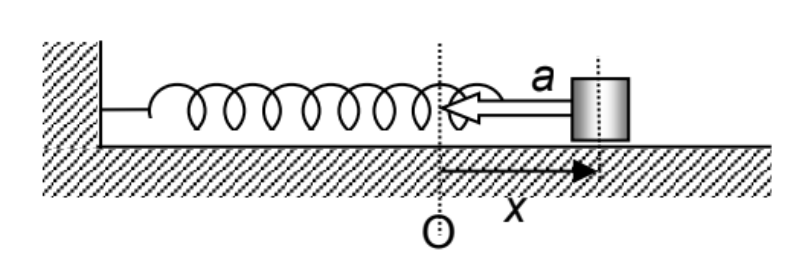
\includegraphics[scale=.4]{assets/mass-spring.png}
	\caption{Mass-spring system}
	\label{fig:mass-spring}
\end{marginfigure}
For a mass-spring system \cref{fig:mass-spring}, the elastic spring force acting on the mass
provides the restoring force, so
\begin{equation*}
	ma = -kx \implies a = -\f{k}{m}x\quad\ab(\omega = \sqrt{\lf{k}{m}})
\end{equation*}

\begin{marginfigure}
	\centering
	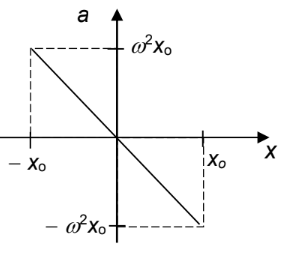
\includegraphics[scale=.7]{assets/shm-ax.png}
	\caption{\(a\) versus \(x\) gives a straight line}
	\label{fig:shm-ax}
\end{marginfigure}
Setting initial conditions as \(x(0) = 0\) and \(v(0) = v_0\), we can get \cref{tab:shm}.
\begin{table}[htpb]
	\centering
	\label{tab:shm}
	\begin{tabular}{c c c}
		\toprule
		qty             & maximum value          & equation                                                     \\
		\midrule
		\(x\)           & \(x_0\)                & \(x = x_0\sin\omega t\)                                      \\
		\(v = \dot{x}\) & \(v_0 = \omega x_0\)   & \(v = \omega x_0\cos\omega t = \pm\omega\sqrt{x_0^2 - x^2}\) \\
		\(a = \dot{v}\) & \(a_0 = \omega^2 x_0\) & \(a = -\omega^2 x_0\sin\omega t\)                            \\
		\bottomrule
	\end{tabular}
	\caption{Equations of s.h.m.}
\end{table}
\begin{marginfigure}
	\centering
	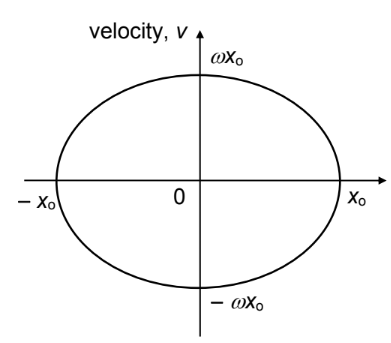
\includegraphics[scale=.6]{assets/shm-vx.png}
	\caption{\(v\) versus \(x\) gives an ellipse}
	\label{fig:shm-vx}
\end{marginfigure}

We can also derive
\begin{align*}
	E_\text{tot} = \max E_k & = \f{1}{2}m{v_0}^2 = \f{1}{2}m\omega^2 {x_0}^2                  \\
	E_k                     & = \f{1}{2}mv^2 = \f{1}{2}m\omega^2 {x_0}^2 \cos^2\omega t       \\
	E_p                     & = E_\text{tot} - E_k = \f{1}{2}m\omega^2 {x_0}^2 \sin^2\omega t
\end{align*}

Between oscillations of the same frequency, the phase difference is
\begin{equation*}
	\Delta\phi = \f{2\pi\Delta t}{T}
\end{equation*}
where \(\Delta t\) is the difference in time to reach the maximum displacement.
Oscillations \bf{in phase} have \(\Delta\phi = 0, 2\pi\), while those \bf{in antiphase} have \(\Delta\phi = \pi\).

\section{Damped oscillations}
\begin{definition}{Damped oscillations}{damped}
	Oscillatory motion in which \it{dissipative forces} cause a progressive decrease in amplitude.
\end{definition}
\begin{figure}[htpb]
	\centering
	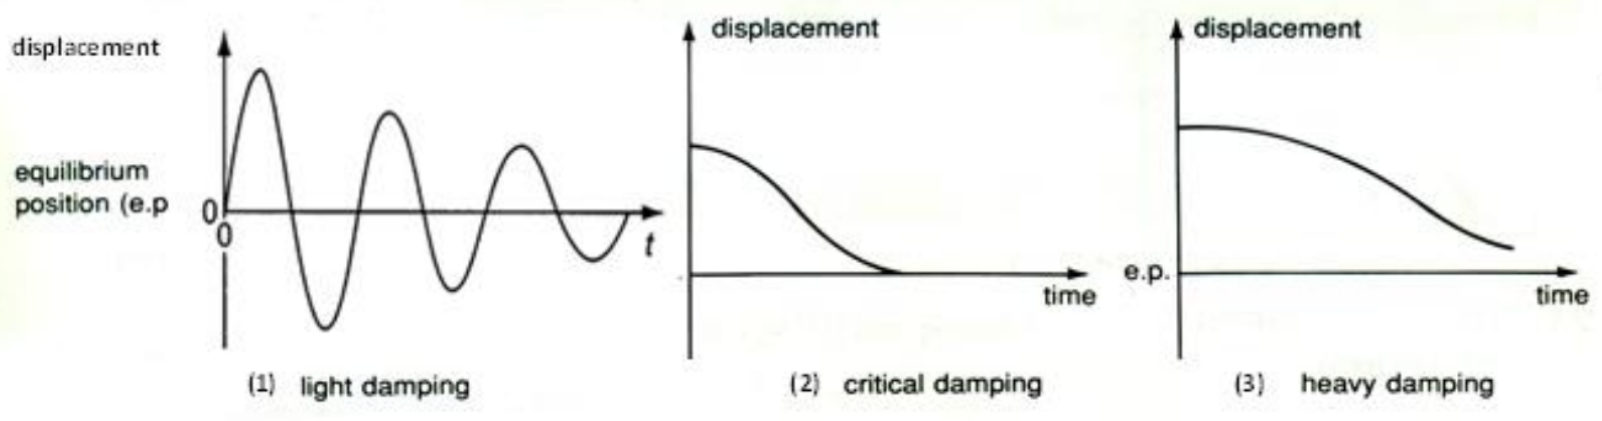
\includegraphics[width=1.1\textwidth]{assets/damping-types.png}
	\caption{Damped oscillations}
	\label{fig:damped}
\end{figure}
\begin{itemize}
	\item \bf{Light damping} causes the amplitude to \it{decrease exponentially with time} across \it{several oscillations} with \it{constant period}.
	\item \bf{Critical damping} causes the system to return to the eq.~pos.~in the shortest possible time without oscillating.
	\item \bf{Heavy damping} or \bf{overdamping} makes the system return to the eq.~pos.~in an infinitely long time.
\end{itemize}

\section{Forced oscillations}
\begin{definition}{Forced oscillations}{forced}
	Oscillatory motion in which an \it{external periodic driving force} is applied to the system.
\end{definition}
\begin{definition}{Resonance}{resonance}
	When the frequency of the external periodic driving force equals the \it{natural frequency} of the system,
	the amplitude of oscillations reaches a maximum.

	This frequency is also the \it{resonant frequency}.
\end{definition}
\begin{marginfigure}
	\centering
	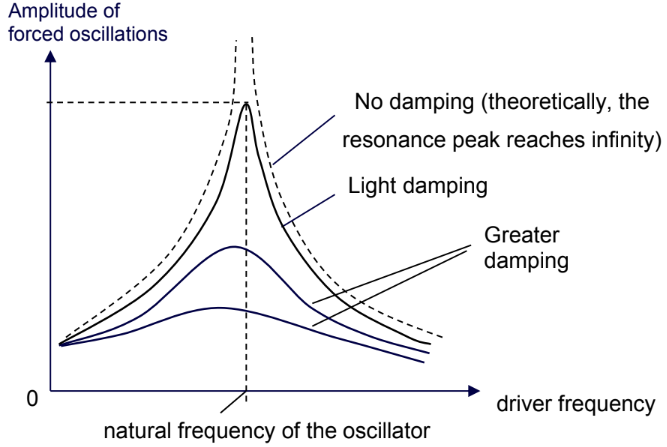
\includegraphics[width=\textwidth]{assets/damped-resonance.png}
	\caption{Resonance in damped system}
	\label{fig:damped-resonance}
\end{marginfigure}
